
\section{Learning Curves}\label{sec:graphs:learning_curves}

Learning curves plots the evaluation metric with respect to a varying training set size. Evaluated with a top-10 recommender list, using F-measure.

\textit{x-axis should it be training size or percent?}

\begin{itemize}
    \item alpha
    \item alpha2
    \item eswc2015movies
    \item eswc2015music
    \item eswc2015books
    \item movielens1m
    \item romeo
\end{itemize}

\Warning[TODO]{ Generate better graphs!! }
\Warning[TODO]{ Why predetermined? Title is WRONG! }


\begin{figure}[ht]
  \centering
    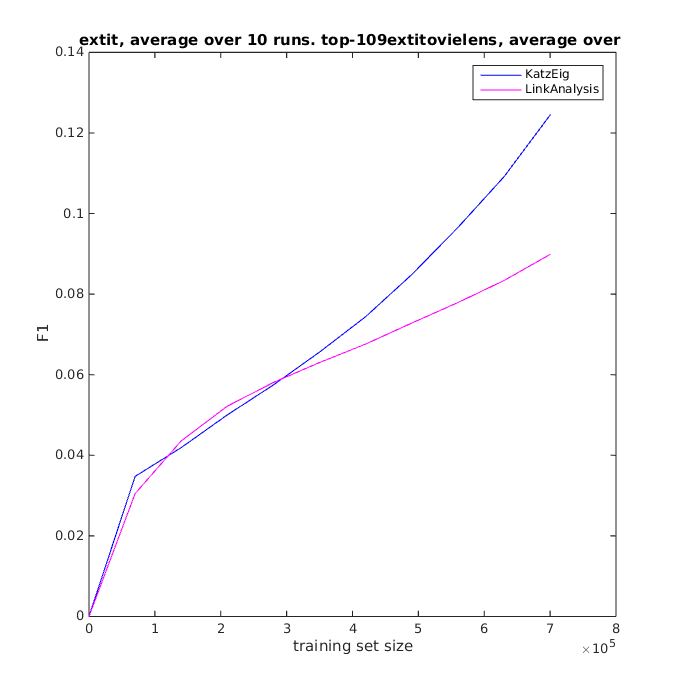
\includegraphics[width=0.9\textwidth]{fig/learning_curves/movielens_learning_curves.png}
    \caption{Learning curves using \textit{movielens1m}
        Used a predetermined $\eta = -2$ and $\gamma = 1.8$ for link-analysis and $\beta = \frac{1}{|A_{train}|}$ with the model $K = 30$ for katz-eig.}
  %\label{fig:sysoverview}
\end{figure}

\begin{figure}[ht]
  \centering
    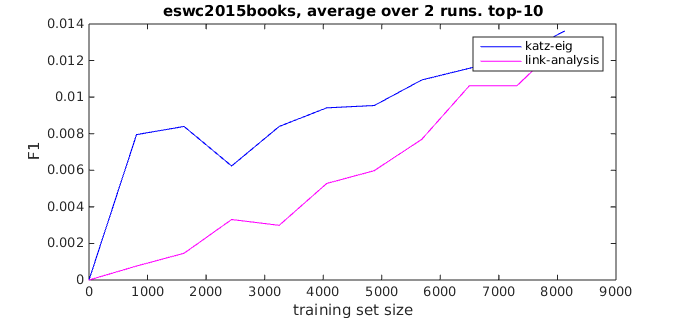
\includegraphics[width=0.9\textwidth]{fig/learning_curves/eswc2015books_learning_curves.png}
    \caption{Learning curves using \textit{eswc2015books}
        Used a predetermined $\eta = -2$ and $\gamma = 1.8$ for link-analysis and $\beta = \frac{1}{|A_{train}|}$ with the model $K = 30$ for katz-eig.}
  %\label{fig:sysoverview}
\end{figure}


%Used a predetermined $\eta = -2$ and $\gamma = 1.8$ for link-analysis and $\beta = \frac{1}{|A_{train}|}$ with the model $K = 10$ for katz-eig.


XXX link-analysis is slower the more training data we have.
katz-eig is practically indifferent.
plot time!

\FloatBarrier
